\documentclass[a4paper, 12pt]{article}
\usepackage[english, russian]{babel}
\usepackage[T2A]{fontenc}
\usepackage{graphicx}
\graphicspath{ {./images/} }

%opening
\title{Web-форум}
\author{Сухинин Сергей\\ 327 группа}

\begin{document}

\maketitle



\section{Описание страниц}
	\subsection{Главная страница}
		К главной странице можно вернуться из любой страницы, нажав соответвующую кнопку в углу
		\begin{itemize}
			\item Кнопки "Вход", "Регистрация", ведущие на соответствующие страницы
			\item Если пользователь авторизовался, то "Вход" и "регистрация" меняются на кнопку, ведущую на страницу аккаунта
			\item Список закрепленных разделов. Какие именно - настраивается админимтратором.
			\item Ссылка на список всех разделов
			\item Модератор имеет доступ к кнопке, ведущей на страницу создания нового раздела
			\item Сыылка на список всех пользователей - участников форума
		\end{itemize}
		
	\subsection{Вход, Регистрация}
		Имеют формы для ввода логина и пароля. Неавторизованный пользователь может читать сообещния в темах, но не может писать сам и создавать новые темы.
		
	\subsection{Аккаунт}
		\begin{itemize}
			\item Настройка данных пользователя
			\item Модератор имеет доступ к управлению блокировками пользователей и правами доступа других пользователей
		\end{itemize}
		
	\subsection{Страница создания раздела}
		Имеет доступ только модератор. Он указывает название раздела и его описание
		
	\subsection{Список пользователей}
		Все пользователи форума. Можно перейти на страницу конкретного пользователя. Присутствует возможность делать выборку по пользоветелям, используя фильтры и раазные варианты сортировки
		
	\subsection{Список разделов}
		Все разделы форума. Можно перейти к конкретному разделу
		
	\subsection{Раздел}
		Представляет из себя список тем в этом разделе, его описание. Можно перейти к конкретной теме. Ссылка на список авторов тем. Ссылка на страницу создания новой темы, доступная всем пользователям
	\subsection{Тема}
		Список сообщений в теме. Отображается автор темы, дата создания. Каждое сообщение - его содержимое, автор, дата публикации, возможные вложения. Есть ссылка на список всех участников темы. По имени автора можно перейти к его странице
		
\section{Навигация страниц}
	Схематичное изображение навигации страниц. Возврат к глайной странице не обозначен, чтобы не нашружать схему лишинми стрелками.
	
	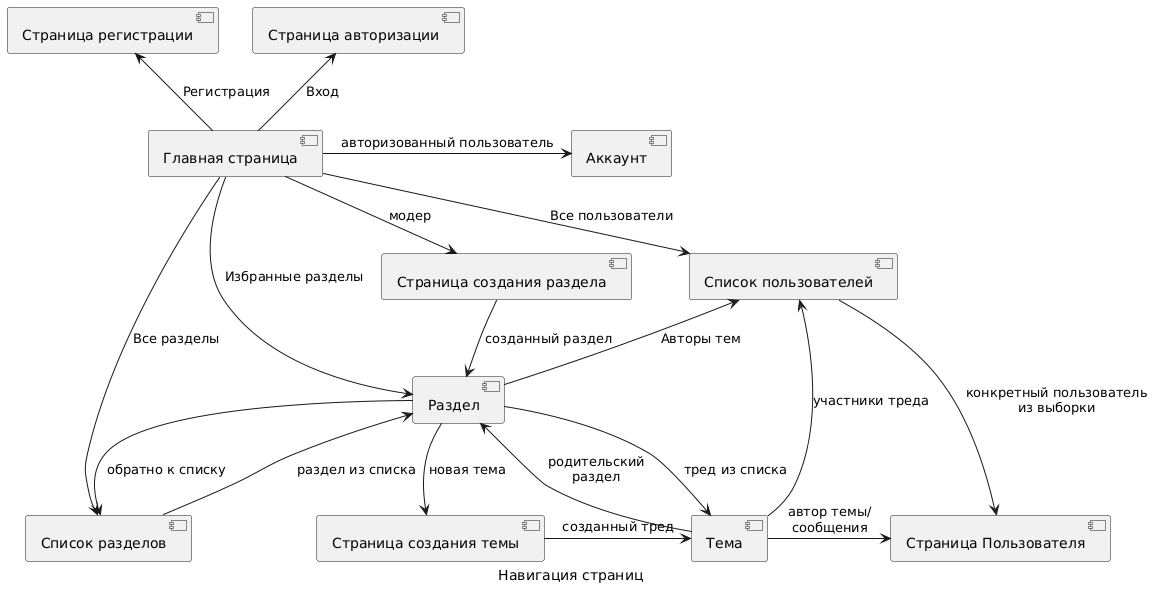
\includegraphics[width=\textwidth]{navigation1}
		
\section{Схема базы данных}
	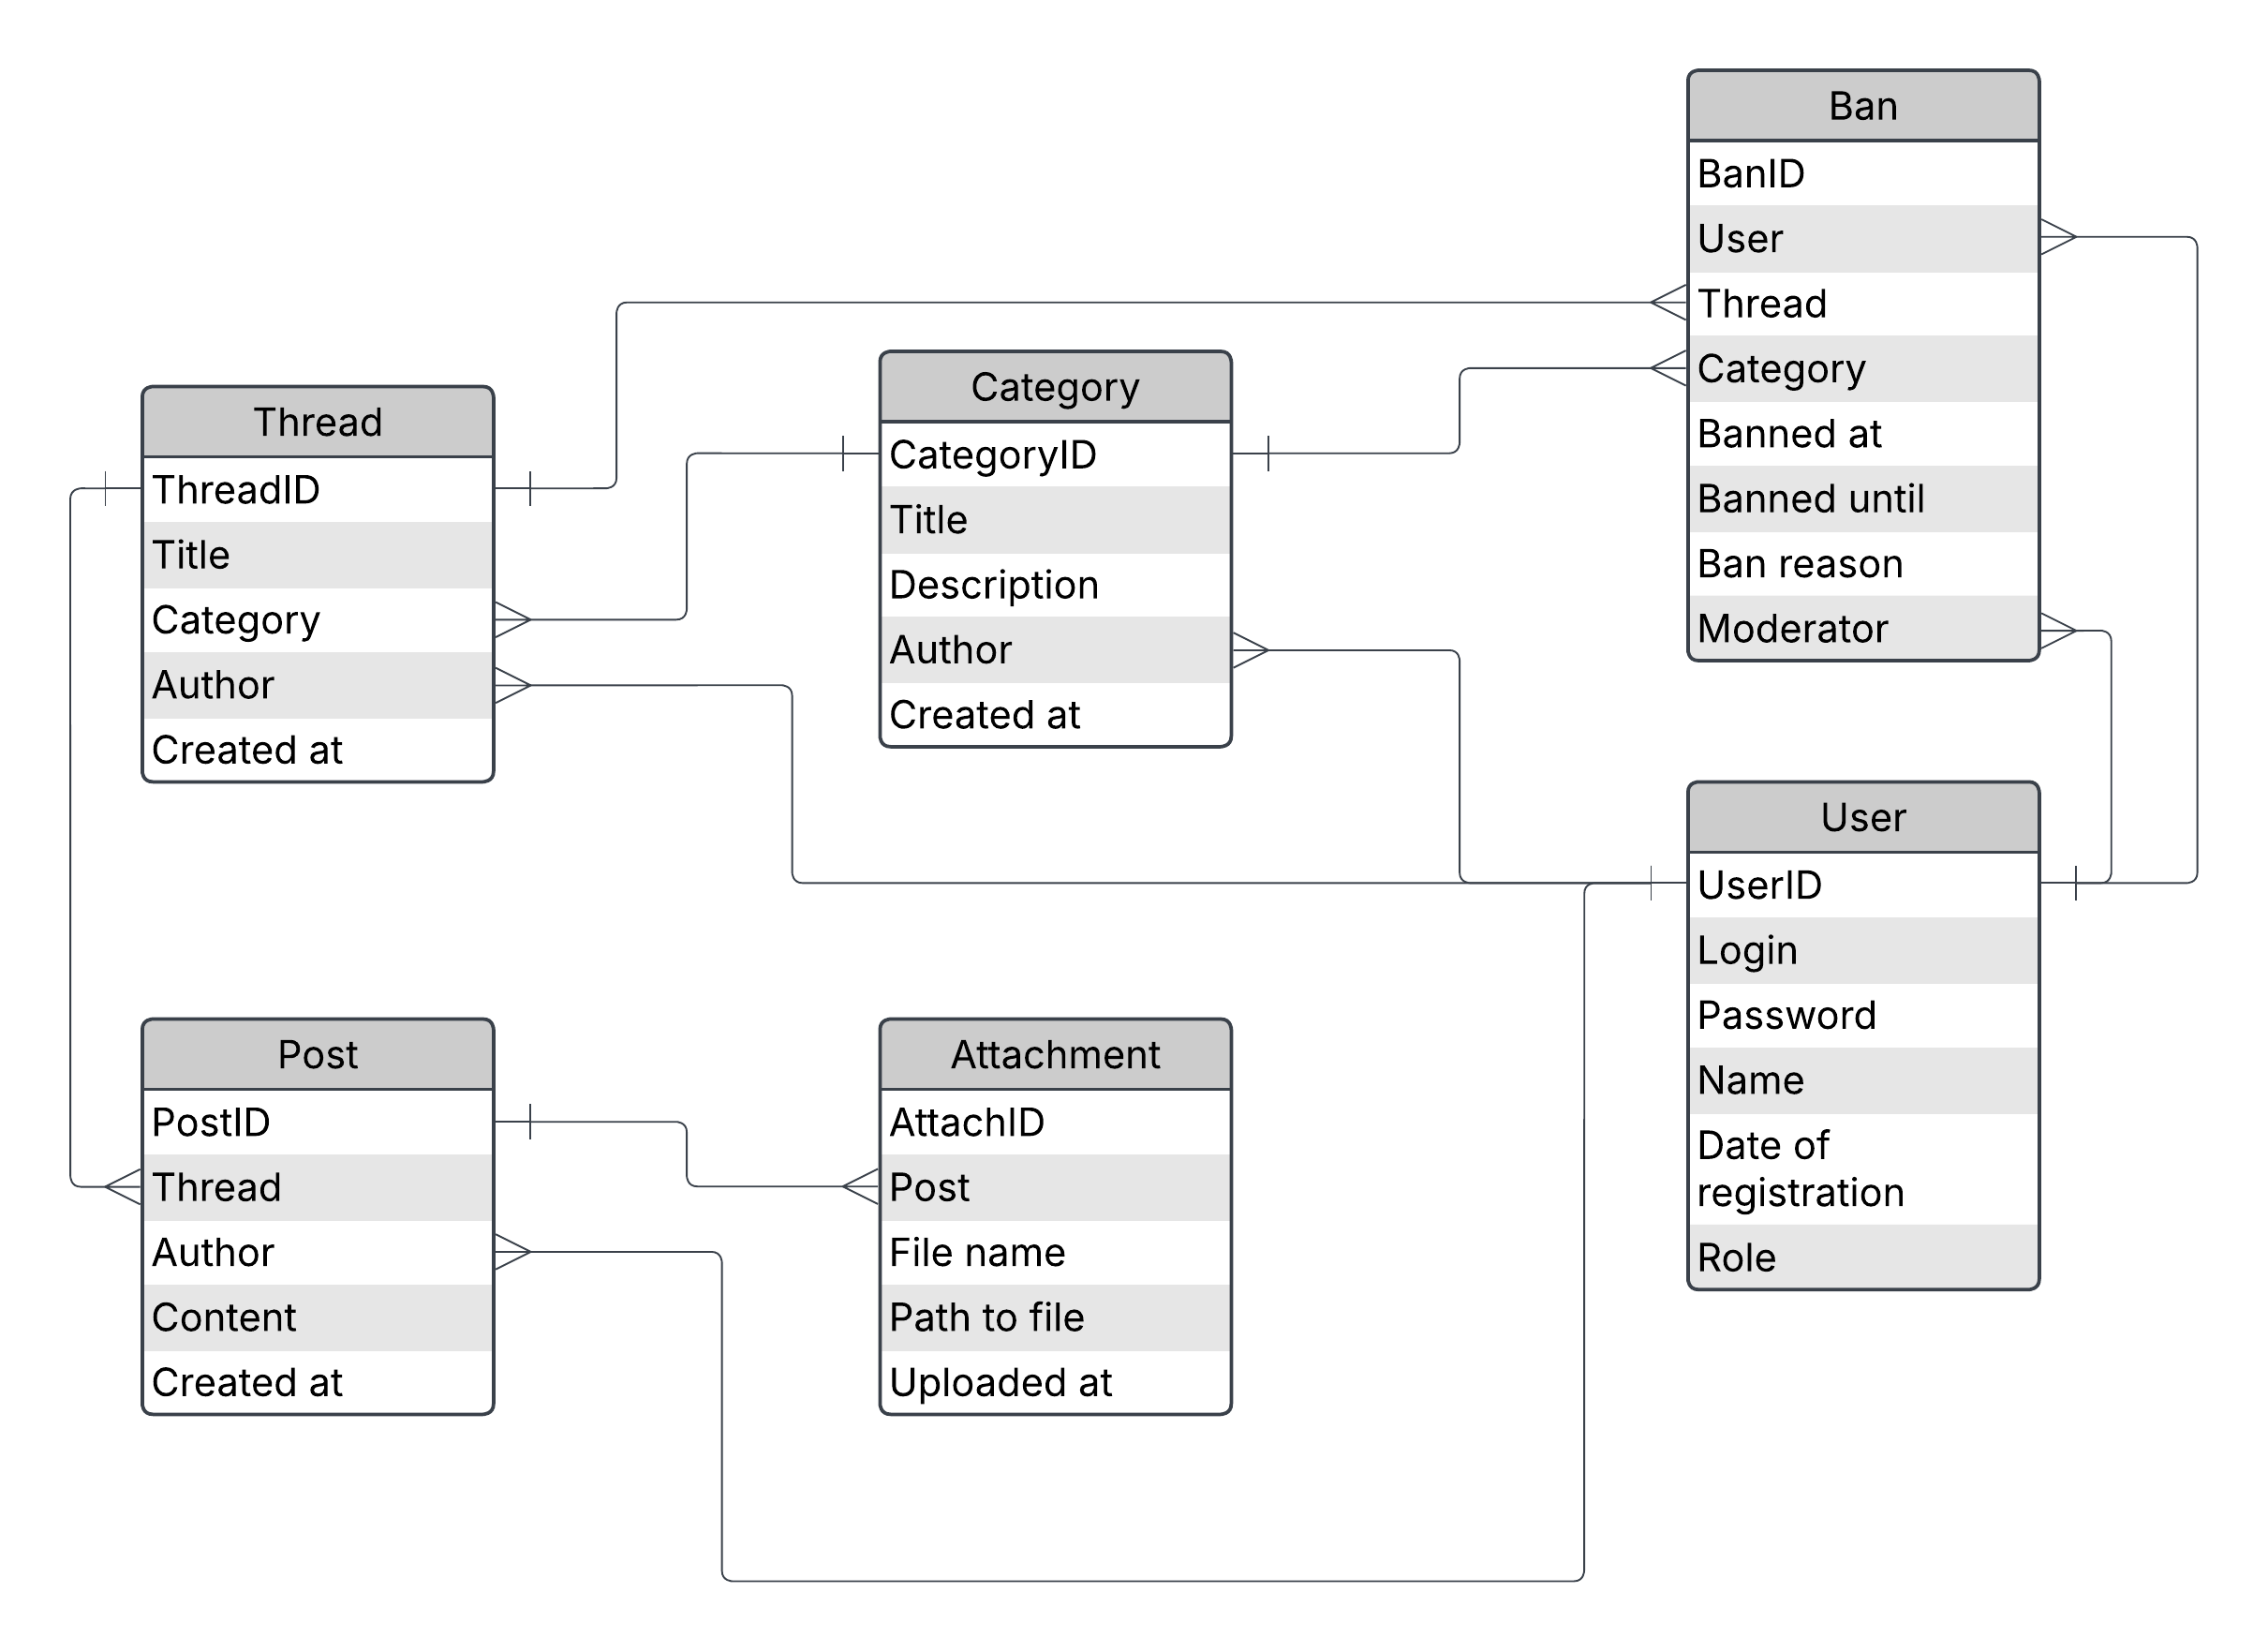
\includegraphics[width=\textwidth]{ERD}
	
\section{Сценарии использования}
	\subsection{Регистрация нового пользователя}
		Создает нового пользователя в базе.
		\begin{enumerate}
			\item Нажать на "Регистрация" на главной странице
			\item Ввести уникальный логин и пароль
			\item Нажать "Зарегистрироваться"
		\end{enumerate}
		
	\subsection{Авторизация}
		Вход в аккаунт
		\begin{enumerate}
			\item Нажать "Вход" на главной странице
			\item Ввести логин существующего пользователя и пароль
			\item Нажать "Войти"
		\end{enumerate}
		
	\subsection{Создание нового раздела}
		Доступно для пользователей с правами модератора
		\begin{enumerate}
			\item Нажать на "Создать новый раздел" на главной странице
			\item Заполнить название нового раздела и его описание
			\item Подтвердить действие. Осуществляется переход на страницу созданного раздела
		\end{enumerate}
		
	\subsection{Выборка пользователей}
		\begin{enumerate}
			\item С главной страницы перейти на страницу со списком всех пользователей
			\item Заполнить поля фильтра(Участие в разделах/темах, дата регистрации и тд)
			\item Выбрать порядок вывода(алфавитный по имени, по дате регистрации, по дате последенго сообщения и тд)
		\end{enumerate}
		
	\subsection{Создание новой темы}
		Доступно всем зарегистрированным пользователям, не имеющим блокировки
		\begin{enumerate}
			\item Перейти в нужный раздел
			\item Нажать кнопку "Создать новую тему"
			\item Ввести название, написать первое сообщение
			\item Подтвердить дейтсвие. Переводит на страницу созданной темы
		\end{enumerate}
		
	\subsection{Сообщение в теме}
		Доступно всем зарегистрированным пользователям, не имеющим блокировки
		\begin{enumerate}
			\item Перейти к нужной теме в разделе
			\item Написать сообщение. Возможно, прикрепить файлы к сообщению
		\end{enumerate}
		
	\subsection{Блокировка пользователя}
		Делает модератор. Можно заблокировать пользователя в определнном разделе, теме или на всем форуме. Блокировка не дает создавать сообщения в заданной теме(в случае блокировки в теме) или создавать новые темы и писать во всех темах в заданном разделе(в случае блокировки в разделе). Блокировка на всем форму запрещает действия во всех разделах. Блокировка может быть на определенный срок или навсегда. Модератор может разблокировать до истечения срока блокировки.
		
	

\end{document}
